\chapter{计算机系统与程序执行的层次}\label{CO01}

\section{系统组成与五大功能部件}\label{CO01-components}

计算机系统由硬件和软件组成。主机通常包含 CPU 与主存；CPU 包含运算器、控制器和寄存器。辅存、输入设备、输出设备合称外部设备。功能部件与物理芯片的划分可不同，一个 CPU 芯片可集成多个核、Cache 和存储控制器。

\par\smallskip
\begin{wideblock}
{\fontsize{9.3}{12}\selectfont\setlength{\tabcolsep}{2.5pt}\setlength{\LTleft}{0pt}\setlength{\LTright}{0pt}
\begin{longtable}{@{}>{\raggedright\arraybackslash}p{\dimexpr0.17930\linewidth-2\tabcolsep\relax}>{\raggedright\arraybackslash}p{\dimexpr0.39077\linewidth-2\tabcolsep\relax}>{\raggedright\arraybackslash}p{\dimexpr0.42994\linewidth-2\tabcolsep\relax}@{}}
\toprule
功能部件 & 基本任务 & 典型状态或部件 \\

\midrule\endfirsthead\toprule
功能部件 & 基本任务 & 典型状态或部件 \\

\midrule\endhead\bottomrule\endfoot
运算器 & 算术、逻辑与移位运算 & ALU、操作数与结果寄存器 \\

控制器 & 取指、译码、产生控制信号、决定后继指令 & PC、IR、控制逻辑 \\

存储器 & 按地址保存指令与数据 & 主存保存执行所需内容，辅存提供大容量非易失空间 \\

输入设备 & 将外部信息转换成机器能处理的形式 & 经接口输入程序和数据 \\

输出设备 & 将内部结果转换成外部所需形式 & 经接口输出数据 \\

\end{longtable}}
\end{wideblock}
\par\smallskip

CPU 数据通路包括寄存器、运算部件及其连接；控制器决定数据流向和操作时刻。早期冯·诺依曼机以运算器为中心，现代组织通常以存储器为中心，外设可经接口、总线和 DMA 与主存交换数据。

\section{存储程序与指令执行}\label{CO01-execution}

存储程序：执行前将指令和数据存入存储器，运行时自动取指、译码、执行。指令与数据均为二进制位串，其用途由当前执行阶段、地址和指令语义确定。冯·诺依曼机由指令控制执行次序，属于控制流驱动。

\par\smallskip
{\fontsize{9.3}{12}\selectfont\setlength{\tabcolsep}{2.5pt}\setlength{\LTleft}{0pt}\setlength{\LTright}{0pt}
\begin{longtable}{@{}>{\raggedright\arraybackslash}p{\dimexpr0.26133\linewidth-2\tabcolsep\relax}>{\raggedright\arraybackslash}p{\dimexpr0.38254\linewidth-2\tabcolsep\relax}>{\raggedright\arraybackslash}p{\dimexpr0.35613\linewidth-2\tabcolsep\relax}@{}}
\toprule
执行阶段 & 地址或数据来源 & 结果 \\

\midrule\endfirsthead\toprule
执行阶段 & 地址或数据来源 & 结果 \\

\midrule\endhead\bottomrule\endfoot
取指 & PC 给出指令地址 & 指令经存储器读入 IR \\

译码与取操作数 & IR 操作码、地址字段及寻址规则 & 确定操作、操作数和有效地址 \\

执行与写回 & 数据通路完成运算、访存或转移 & 更新寄存器、存储器和标志 \\

后继地址形成 & 顺序地址或转移、调用、异常入口 & 更新 PC，继续取指 \\

\end{longtable}}
\par\smallskip

PC 的顺序增量由地址单位和指令长度决定：按字节编址、定长 4 B 指令时通常加 4。流水线可使多条指令的各阶段重叠；程序可见效果仍须符合 ISA。

MAR 保存本次主存访问地址，MDR 保存本次交换的位串；二者可在不同阶段分别传送指令地址、数据地址以及指令、数据。

\subsection{\texorpdfstring{程序 \(y=ab+c\) 的寄存器状态}{程序 y=ab+c 的寄存器状态}}\label{CO01-program}

按字编址，地址 0～4 存取数、乘法、加法、存数和停机指令，地址 5～8 存 \(a=2,b=3,c=1,y=0\)。

\par\smallskip
{\fontsize{9.3}{12}\selectfont\setlength{\tabcolsep}{2.5pt}\setlength{\LTleft}{0pt}\setlength{\LTright}{0pt}
\begin{longtable}{@{}>{\raggedright\arraybackslash}p{\dimexpr0.24744\linewidth-2\tabcolsep\relax}>{\raggedright\arraybackslash}p{\dimexpr0.38889\linewidth-2\tabcolsep\relax}>{\raggedright\arraybackslash}p{\dimexpr0.36367\linewidth-2\tabcolsep\relax}@{}}
\toprule
指令地址 & 数据操作 & 完成状态 \\

\midrule\endfirsthead\toprule
指令地址 & 数据操作 & 完成状态 \\

\midrule\endhead\bottomrule\endfoot
0 & \(M[5]\to\mathrm{ACC}\) & ACC=2，后继地址1 \\

1 & \(\mathrm{ACC}\times M[6]\to\mathrm{ACC}\) & ACC=6，后继地址2 \\

2 & \(\mathrm{ACC}+M[7]\to\mathrm{ACC}\) & ACC=7，后继地址3 \\

3 & \(\mathrm{ACC}\to M[8]\) & \(M[8]=7\)，后继地址4 \\

4 & 停机 & 计算结束 \\

\end{longtable}}
\par\smallskip

\begin{figure}[H]
\centering
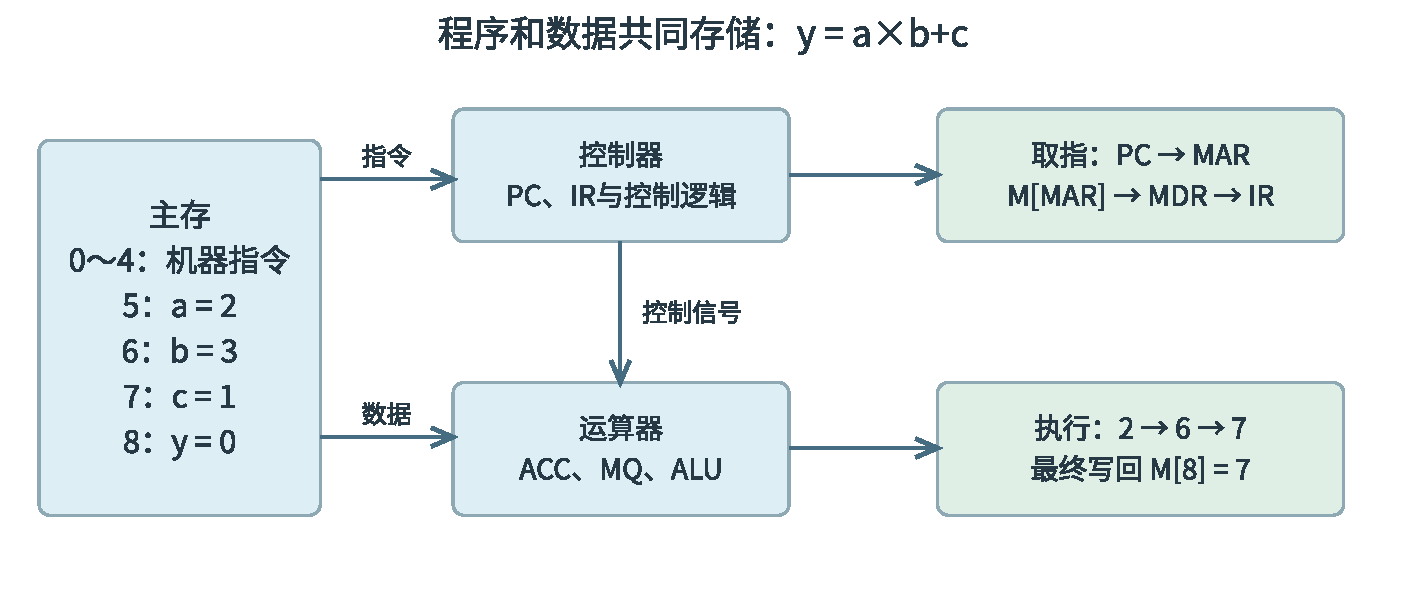
\includegraphics[width=\linewidth,height=108mm,keepaspectratio]{figures/CO01_program_path.pdf}
\caption{主存按地址保存程序与数据，控制器组织取指与执行}
\end{figure}

示意机器中 ACC 暂存操作数或结果，MQ 辅助保存乘数或乘积低位，X 暂存另一个输入。具体寄存器配置以题设数据通路为准。

\section{ISA、系统层次与软件}\label{CO01-architecture}

\par\smallskip
\begin{wideblock}
{\fontsize{9.3}{12}\selectfont\setlength{\tabcolsep}{2.5pt}\setlength{\LTleft}{0pt}\setlength{\LTright}{0pt}
\begin{longtable}{@{}>{\raggedright\arraybackslash}p{\dimexpr0.37237\linewidth-2\tabcolsep\relax}>{\raggedright\arraybackslash}p{\dimexpr0.62763\linewidth-2\tabcolsep\relax}@{}}
\toprule
对象 & 规定或提供的内容 \\

\midrule\endfirsthead\toprule
对象 & 规定或提供的内容 \\

\midrule\endhead\bottomrule\endfoot
ISA（指令集体系结构） & 软件可见的指令功能与编码、寄存器、数据类型、寻址方式和存储访问规则 \\

微体系结构 & ISA 的内部实现：流水级、转发、Cache 组织、加法器结构等 \\

操作系统 & 资源管理、进程运行环境和服务接口 \\

系统软件 & 操作系统、语言处理程序、数据库管理系统、相关工具和库 \\

应用软件 & 面向用户具体任务的程序 \\

\end{longtable}}
\end{wideblock}
\par\smallskip

相同 ISA 可由不同微体系结构实现，具有不同 CPI。机器码执行还受操作系统、ABI、库及可执行文件格式约束。软硬件逻辑功能等价表示同一功能可由软件算法或专用硬件实现，选择取决于时间、空间、成本、功耗与可修改性。

常用抽象层次自下而上为微程序机器级、传统机器语言级、操作系统级、汇编语言级、高级语言级。微程序级适用于采用微程序控制的机器。``透明''表示上层使用者无需处理下层实现细节。

\subsection{程序翻译与装入}\label{CO01-translation}

\[\begin{aligned}
\text{源程序}&\xrightarrow{\text{预处理}}\text{展开后的源程序}\\
&\xrightarrow{\text{编译}}\text{汇编程序}\xrightarrow{\text{汇编}}\text{可重定位目标文件}\\
&\xrightarrow{\text{链接}}\text{可执行文件}.
\end{aligned}\]

预处理展开头文件、宏等；链接合并目标与库，完成符号解析和重定位；装入建立进程地址空间并准备执行入口。宏和伪指令可展开为零条、一条或多条机器指令，一条高级语言语句与机器指令条数无固定对应关系。

解释器在运行时读取源程序或中间表示并完成操作，解释器自身由机器指令运行。语言实现可组合解释、预编译和即时编译。

\par\medskip\Needspace{4\baselineskip}\noindent\hypertarget{CO01-E01}{}\label{CO01-E01}\textbf{例 1-1}\par\nobreak\smallskip

计算机硬件能够直接执行的是（　）。

I. 机器语言程序　II. 汇编语言程序　III. 硬件描述语言程序

A. 仅 I　 B. 仅 I、II　 C. 仅 I、III　 D. I、II、III

\section{字长、编址与容量}\label{CO01-capacity}

\par\smallskip
{\fontsize{9.3}{12}\selectfont\setlength{\tabcolsep}{2.5pt}\setlength{\LTleft}{0pt}\setlength{\LTright}{0pt}
\begin{longtable}{@{}>{\raggedright\arraybackslash}p{\dimexpr0.32205\linewidth-2\tabcolsep\relax}>{\raggedright\arraybackslash}p{\dimexpr0.67795\linewidth-2\tabcolsep\relax}@{}}
\toprule
名称 & 含义 \\

\midrule\endfirsthead\toprule
名称 & 含义 \\

\midrule\endhead\bottomrule\endfoot
机器字长 & CPU 一次整数运算通常能处理的基本位宽 \\

存储字长 & 一个存储单元保存的位数 \\

指令字长 & 一条指令编码所占位数，可定长或变长 \\

MAR 位数 & 可编码的主存地址位数 \\

MDR 位数 & 一次主存数据交换的位宽 \\

\end{longtable}}
\par\smallskip

若 \(m\) 位完整地址全部可用，每个地址对应 \(w\) 位，则容量为 \(2^m w\) bit。按字节编址时为 \(2^m\) B。已安装物理容量可以小于可编址空间。

\begin{itemize}
\tightlist
\item
  20 位字节地址：1 MiB；20 位、16 位字地址：2 MiB。
\item
  \(2^{10}\) 个16位单元：2 KiB；按字编址需10位，改为按字节编址需11位。
\item
  4 KiB 主存、存储字长32位：按字编址需10位，按字节编址需12位。
\end{itemize}

容量常用 \(1\mathrm{KiB}=2^{10}\mathrm B\)、\(1\mathrm{MiB}=2^{20}\mathrm B\)；频率、速率的 k、M、G 通常按 \(10^3,10^6,10^9\)。带宽为每次传送字节数乘每秒传送次数，单位进制服从题设。

\section{CPU 执行时间与性能指标}\label{CO01-performance}

响应时间为从请求到得到结果的总历时；吞吐量为单位时间完成的任务量。程序总时间可包含 CPU 工作、I/O 等待和调度等。CPU 时间按实际动态执行的指令计算。

设第 \(i\) 类指令执行 \(n_i\) 条、平均占 \(c_i\) 个周期，主频为 \(f\)：

\[N=\sum_i n_i,\qquad C=\sum_i n_i c_i,\qquad\overline{\mathrm{CPI}}=\frac{C}{N}=\sum_i\frac{n_i}{N}c_i,\]

\[T_{\mathrm{CPU}}=\frac{N\overline{\mathrm{CPI}}}{f}=N\overline{\mathrm{CPI}}T_{\mathrm{clk}},\qquad T_{\mathrm{clk}}=\frac1f.\]

平均 CPI 以指令条数为权重；Cache 缺失、流水停顿等也计入统计范围内的周期。多发射处理器的平均 CPI 可以小于1，单条指令仍可能经历多个周期的延迟。

\par\smallskip
\begin{wideblock}
{\fontsize{9.3}{12}\selectfont\setlength{\tabcolsep}{2.5pt}\setlength{\LTleft}{0pt}\setlength{\LTright}{0pt}
\begin{longtable}{@{}>{\raggedright\arraybackslash}p{\dimexpr0.38962\linewidth-2\tabcolsep\relax}>{\raggedright\arraybackslash}p{\dimexpr0.61038\linewidth-2\tabcolsep\relax}@{}}
\toprule
指标 & 定义及计算条件 \\

\midrule\endfirsthead\toprule
指标 & 定义及计算条件 \\

\midrule\endhead\bottomrule\endfoot
IPC & 每周期平均完成指令数；同一统计区间下 \(\mathrm{IPC}=1/\overline{\mathrm{CPI}}\) \\

MIPS & 每秒百万条指令，\(f/(\overline{\mathrm{CPI}}\times10^6)\) \\

MFLOPS／GFLOPS／TFLOPS & 每秒浮点运算数分别除以 \(10^6/10^9/10^{12}\) \\

同一任务性能比 & \(P_A/P_B=T_B/T_A\) \\

\end{longtable}}
\end{wideblock}
\par\smallskip

不同 ISA、编译器和优化方案可改变动态指令数与指令组成。比较同一任务优先使用实际执行时间，主频、CPI、MIPS 和字长各自只描述部分条件。

\par\medskip\Needspace{4\baselineskip}\noindent\hypertarget{CO01-E02}{}\label{CO01-E02}\textbf{例 1-2}\par\nobreak\smallskip

某计算机主频为1 GHz，程序 P 运行过程中共执行10000条指令，其中80\%的指令执行平均需1个时钟周期，20\%的指令执行平均需10个时钟周期。程序 P 的平均 CPI 和 CPU 执行时间分别是（　）。

A. 2.8，28 μs　 B. 28，28 μs　 C. 2.8，28 ms　 D. 28，28 ms

\subsection{性能变化的时间比}\label{CO01-ratio}

同一任务，前后两方案满足同一 CPU 时间模型时：

\[\frac{T'}{T}=\frac{N'}N\frac{\mathrm{CPI}'}{\mathrm{CPI}}\frac f{f'}.\]

编译优化可同时改变 \(N\) 与 CPI；Cache 改进通常减少停顿；升频还可能伴随 CPI 变化。若20 s程序指令数变为70\%、CPI变为1.2倍且主频不变，时间为 \(20\times0.7\times1.2=16.8\) s。

\section{局部加速与 Amdahl 定律}\label{CO01-amdahl}

原时间中比例 \(p\) 的部分加快为原速度的 \(s\) 倍，其他部分不变，各部分时间可相加且无新增开销时：

\[T'=T[(1-p)+p/s],\qquad S=\frac T{T'}=\frac1{(1-p)+p/s}.\]

当 \(s\to\infty\) 且 \(p<1\)，加速比上限为 \(1/(1-p)\)。``速度提高50\%''对应 \(s=1.5\)。计算与 I/O 重叠、通信或同步开销变化时，先按实际时间关系重新建模。

\par\medskip\Needspace{4\baselineskip}\noindent\hypertarget{CO01-E03}{}\label{CO01-E03}\textbf{例 1-3}\par\nobreak\smallskip

假定基准程序 A 在某计算机上的运行时间为100 s，其中90 s为 CPU 时间，其余为 I/O 时间。若 CPU 速度提高50\%，I/O 速度不变，则运行基准程序 A 所耗费的时间是（　）。

A. 55 s　 B. 60 s　 C. 65 s　 D. 70 s

增加处理器可让独立任务并发，提高吞吐量。两个各需单核2 s的任务在双核上同时开始，全部完成历时可由4 s变为2 s；每个无排队任务的执行时间仍为2 s。

\section{器件发展阶段}\label{CO01-history}

电子管 \ensuremath{\to} 晶体管 \ensuremath{\to} 中小规模集成电路 \ensuremath{\to} 大规模与超大规模集成电路。集成度提高推动可靠性、容量、速度和微型化、多核与并行计算发展。摩尔定律描述晶体管数量增长的历史经验趋势，程序加速仍由具体执行时间模型判断。
